\documentclass[UTF8,fontset=none,11pt]{ctexart}
\setCJKmainfont[ItalicFont={Noto Serif CJK SC},ItalicFeatures={FakeSlant=0.15}]{Noto Serif CJK SC}\setCJKsansfont{Noto Sans CJK SC}\setCJKmonofont{Noto Sans Mono CJK SC}
\usepackage[a4paper,margin=25mm,top=22mm,bottom=22mm]{geometry}
\usepackage{amsmath,amssymb,amsthm,mathtools,booktabs,array,graphicx,xcolor,hyperref,microtype,fancyhdr}
\definecolor{ink}{HTML}{183448}\hypersetup{colorlinks=true,linkcolor=ink,citecolor=ink,urlcolor=ink,pdfauthor={},pdftitle={Uniform average mixing on paths}}
\newtheorem{theorem}{Theorem}\newtheorem{lemma}[theorem]{Lemma}\newtheorem{corollary}[theorem]{Corollary}
\theoremstyle{remark}\newtheorem*{remark}{Remark}
\newcommand{\E}{\mathbb E}\newcommand{\R}{\mathbb R}\newcommand{\Z}{\mathbb Z}\newcommand{\Q}{\mathbb Q}\newcommand{\T}{\mathbb T}\newcommand{\abs}[1]{\left|#1\right|}\newcommand{\norm}[1]{\left\|#1\right\|_1}
\DeclareMathOperator{\conv}{conv}\DeclareMathOperator{\ri}{ri}\DeclareMathOperator{\diag}{diag}\DeclareMathOperator{\Rea}{Re}
\pagestyle{fancy}\fancyhf{}\fancyhead[L]{\small Uniform average mixing on paths}\fancyhead[R]{\small Research preprint v0.1.0}\fancyfoot[C]{\thepage}\setlength{\headheight}{15pt}\setlength{\parindent}{1.2em}\setlength{\parskip}{1.5pt}\allowdisplaybreaks

\fancyhead[L]{\small 路径图的均匀平均混合}\fancyhead[R]{\small 研究预印本 v0.1.0}
\title{\vspace{-1.2em}\bfseries 路径图均匀平均混合的算术分类：\\基于正 Fourier 概率密度的证明方法}
\author{}\date{2026 年 11 月 27 日 \quad $\cdot$ \quad 研究预印本 v0.1.0}
\begin{document}\maketitle
\begin{center}\small AI 辅助研究稿；候选证明，尚未经独立同行评议。\end{center}
\begin{abstract}
对于 $N$ 顶点路径图上的连续时间邻接量子行走，均匀平均混合要求存在同一读出时间概率分布，使平均跃迁矩阵为 $J_N/N$。令 $q=N+1$。Kang 已证明当 $15\mid q$、$21\mid q$ 或 $6\mid q$ 且 $q\ge12$ 时均匀平均混合不存在，并证明了素数、两倍素数和 2 的幂次模数的存在性。本文提出覆盖其余全部情形的候选充分性证明。通过将能谱整数关系转化为圆分域上的有符号单位根消失和，利用低阶 Fourier 矩和严格正概率密度构造，在独立相位模型、三坐标校验块模型及奇偶性相位群上分别实现目标相干矩。原先依赖线性规划证书的 13 个偶数模数和 $q=33$ 现均采用精确有理数 Fourier 计算处理，其他小奇数模数另行证明。进一步得到预设代数步长时间网格上的有限支撑存在性，以及条件性的统一 Haar 成分和已知时间噪声补偿界。本文是英文研究主稿的中文配套稿，完整短关系分类和逐项计算细节见同包英文补充证明。全部分类尚未经独立同行审查或完整 Lean 形式化。
\end{abstract}
\noindent\textbf{关键词：} 连续时间量子行走；均匀平均混合；圆分域；Fourier 矩；凸几何。
\section{引言与主要结论}
设 $A$ 为 $N\ge2$ 顶点路径图 $P_N$ 的邻接矩阵。归一化的单粒子哈密顿量为 $A$，跃迁概率矩阵为 $M(t)=|e^{itA}|^{\circ2}$，其中 $\circ$ 表示逐元素运算。对 Borel 概率测度 $\mu$，定义
\begin{equation}\label{zh:mix}\widehat M[\mu]=\int_{\R} M(t)\,d\mu(t).\end{equation}
均匀平均混合要求 $\widehat M[\mu]=J_N/N$。同一时间分布必须适用于所有初态位置。这不同于单一时刻的瞬时均匀混合，也不同于通常的 Ces\`aro 长时间平均\cite{godsil}。Baptista 等\cite{baptista}研究了随机时间平均并给出小路径图例子；Kang\cite{kang}建立了强制相干矩条件和奇偶性能隙碰撞分类。不存在碰撞仅表明目标相干矩相容，仍须构造合法概率分布。
\begin{theorem}[候选完整算术分类]\label{zh:main}
令 $q=N+1\ge3$，则 $P_{q-1}$ 存在均匀平均混合当且仅当
\begin{equation}15\nmid q,\qquad21\nmid q,\qquad 6\nmid q\ \text{或}\ q=6.\end{equation}
对每个允许的 $q$，任取正代数数 $\delta$ 和 $t_0\ge0$，可在 $t_0+\delta\Z_{\ge0}$ 中选取有限个时间构成严格混合协议。令 $m=\lfloor(q-1)/2\rfloor$，奇数模数支撑数不超过 $m^2+1$，偶数模数不超过 $m(m+1)+1$。
\end{theorem}
必要性来自文献\cite{kang}的定理 S18；本文的候选贡献是剩余充分性。证明分为三类：不含 3 的奇数模数、含 3 且与 35 互素的奇数模数，以及不含 3 的偶数模数。$q=6$ 是已有正例。图~\ref{zh:class}展示了前 210 个模数的分类情况。英文主稿（\texttt{paper-en.pdf}）及详细证明（\texttt{detailed-proof.md}，下称 DP）共同给出完整论证；尤其 DP 的短关系分类属于证明不可缺少的组成部分。
\begin{figure}[ht]\centering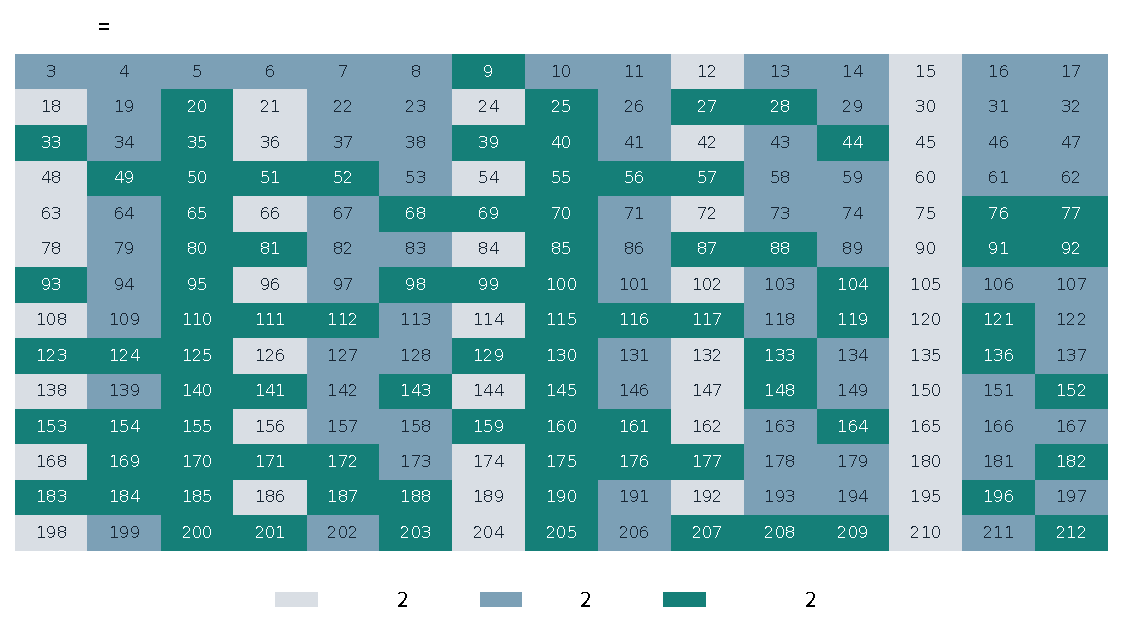
\includegraphics[width=.98\linewidth]{../figures/classification-zh.pdf}\caption{从 $q=3$ 开始的 210 个模数的算术分类示意。浅灰为已知否定类，蓝色为已知正例，深青色为本研究拟补充的正例。分类图仅作展示，并非穷尽证明。}\label{zh:class}\end{figure}
\section{谱分解与目标相干矩}
路径图能谱和本征矢分别为
\begin{equation}\theta_r=2\cos(r\pi/q),\quad v_r(k)=\sqrt{2/q}\sin(rk\pi/q),\quad E_r=v_rv_r^{\mathsf T}.\end{equation}
记反射矩阵为 $S$，单位矩阵为 $I$，全一矩阵为 $J$。由谱分解，
\begin{align}M(t)&=D_0+2\sum_{r<s}\cos[(\theta_r-\theta_s)t]E_r\circ E_s,\\D_0&=\sum_r E_r\circ E_r=\frac{2J+I+S}{2q}.\end{align}
镜像奇偶性投影算符为 $(I\pm S)/2$，其逐元素平方之和为 $(I+S)/2$。因此对任意 $r\ne s$，若能实现
\begin{equation}\label{zh:coh}y_{rs}=\E\cos[(\theta_r-\theta_s)T]=\begin{cases}-1/N,&r\equiv s\pmod2,\\0,&r\not\equiv s\pmod2,\end{cases}\end{equation}
则平均跃迁矩阵即为 $D_0-N^{-1}[(I+S)/2-D_0]=J/N$。文献\cite{kang}进一步证明了这些相干系数的唯一性及禁止模数的完整碰撞分类。

每个正负能谱对选取一个非零能级代表。奇数 $q$ 时取 $\alpha_j=2\cos(2\pi j/q)$，$1\le j\le m$（不要求它们均为正）；偶数 $q$ 时取 $\alpha_j=\theta_j$，$j<q/2$。令 $z_j=e^{i\phi_j}$，定义紧致相位群及整数关系格
\begin{equation}H=\overline{\{t\alpha\bmod2\pi:t\in\R\}},\qquad \Lambda=\{c\in\Z^m:c\cdot\alpha=0\}.\end{equation}
归一化 Haar 测度 $h$ 满足 $\int_H z^c\,dh=\mathbf1_{c\in\Lambda}$。关键是构造满足式~\eqref{zh:coh}的相位概率测度。
\begin{lemma}[Fourier 修正引理]\label{zh:lemma}
设目标特征 $V$ 非平凡且两两不互为逆或相等。对非负实 Fourier 多项式 $F$，定义 $Z_H=\E_hF$、$M_v=\E_h(F\Rea z^v)$。给定目标 $y_v$ 与 $T>0$，
\begin{equation}\label{zh:f}f=\frac{F+T-Z_H+2\sum_{v\in V}(Ty_v-M_v)\Rea z^v}{T}\end{equation}
的积分为 1，目标矩为 $y_v$；若 $T-Z_H>2\sum_v|Ty_v-M_v|$，则 $f$ 严格为正。
\end{lemma}
\begin{proof}Haar 正交关系给出各目标余弦均值为零、平方积分为 $1/2$、不同余弦的内积为零。对式~\eqref{zh:f}及其与目标余弦的乘积积分即得。利用 $F\ge0$ 和 $|\Rea z^v|\le1$ 得到正性下界。\end{proof}
\section{短能谱关系的全局归约}
多项式 $F$ 的 Fourier 次数不超过 8，乘上二阶目标矩后只涉及 $\norm c\le10$ 的整数关系。相应有符号单位根数组绝对权重不超过 20。将其非零支撑划分为保持原有系数的极小消失子集。Conway--Jones 定理\cite[定理5]{cj}（另见 Lenstra\cite[定理2.6]{lenstra}）说明每个极小关系的约化阶数 $d$ 无平方因子，支撑至少为
\begin{equation}2+\sum_{p\mid d}(p-2).\end{equation}
对于偶数 $q$，令 $\zeta=e^{i\pi/q}$，利用 $\zeta^{j+q}=-\zeta^j$ 将指数折叠到模 $q$。所用的 $\pm r$（$0<r<q/2$）在模 $q$ 下互不相同，因此不会合并支撑。约化阶数的因子 2 可以吸收入符号，剩余阶数为奇数。反演不动的奇阶陪集包含唯一不动点：奇数模数时为 0，偶数模数时为 0 或 $q/2$。后者中心提升因子分别为 $1$ 与 $i$，得到对称和反对称数组。支撑大于 10 的极小关系必须在中心陪集，否则反演后的不交陪集还需超过 10 个支撑点。

另一种独立归约使用圆分多项式。若 $d$ 是 $q$ 的奇数根基，$a=q/d$，则奇数情形 $\Phi_q(x)=\Phi_d(x^a)$，偶数情形 $\Phi_{2q}(x)=\Phi_{2d}(x^a)$。将数组多项式按模 $a$ 的指数分块，各块须分别满足圆分整除条件。平方自由阶数 $d=pr$ 的 $p$ 行求值在 $\Q(\zeta_r)$ 中必须相同；若 $p>20$，至少一行为空，因而各行都单独消失。这表明高次幂和大素因子不产生额外局部短关系模板。进一步的局部分类仍然是必要的，不能仅靠这一归约得出充分性。

当全部奇素因子不小于 5 时，可能的复合约化阶数仅有 $35,55,65,77,85,91,385$；当素因子仅为 3 和不小于 11 的素数时，仅有 $33,39,51,57$。对于两素数阶数 $pr$，中国剩余定理把关系表示为矩形数组 $A_{ij}=a_i+b_j$：行列常值数组的维数 $p+r-1$ 恰为圆分求值核的维数。中心数组 $a_0=b_0=0$。若两轴非零支撑为 $u,v$，则至少有 $u(r-v)+(p-u)v$ 个非零项；反对称情形另有至少 $uv/2$ 个交叉项。对 $35$ 阶的对称数组，半权重为
\[L=|a_1|+|a_2|+\sum_{j=1}^3(|b_j|+2|a_1+b_j|+2|a_2+b_j|).\]
当 $L\le10$ 且 $a_1\ne a_2$ 时，交换及整体变号后只需考虑 $(0,1)$，$b_j\in\{0,-1\}$。相等的非零轴值只能为 $\pm1,\pm2$；反对称的列代价为 $|b|+2\max(|a_1|,|b|)+2\max(|a_2|,|b|)$，两轴非零时仅有一个单位行轴和单位列轴。由此得到 44 个对称和 24 个反对称混合数组（含正负号）。

对 $385$ 阶，极小支撑至少 19，结合反演与权重预算得到恰好 20 个单位系数项。将其分成 11 个 $5\times7$ 切片，所有切片求值相同且非零，至少两片仅含一个单位根。反对称中心要求公共值为纯虚数，与奇阶单位根矛盾。对称中心可整体变号令公共值为 1，非单项切片至少含 4 项。剩余支撑只允许中心 4 项加一对各 4 项的切片，或中心 10 项。前者降为 55 阶；后者的加法数组半权重不可能为 5。完整逐类排除、系数计数和正性界的依据见 DP 的三个证明部分及英文主稿引理 3。这里未将有限枚举结果外推为一般结论。
\section{三类正概率密度}
\subsection{不含 3 的奇数模数}
此时 $m=(q-1)/2$，目标为 $\E\Rea(z_i\bar z_j)=-1/(2m)$（$i<j$）及 $\E\Rea(z_i z_j)=0$（$i\le j$）。令
\begin{equation}X=\frac1m\left|\sum_j z_j\right|^2,\qquad F=(100-60X+7X^2)^2.\end{equation}
独立圆周模型下，$Z=\E_*F$、$Y=\E_*XF$，且
\[\E_*X^k=\frac{(k!)^2}{m^k}[t^k]\left(\sum_{j=0}^k\frac{t^j}{(j!)^2}\right)^m.\]
取 $T=2m(Z-Y)/(m-1)$，当 $m\ge3$ 时可用正性裕量为
\[G=T-Z=\frac{3(232m^3+2568m^2-5782m+15435)}{m^3}\ge696.\]
相关短关系的长度为偶数、荷数 $Q(c)=\sum c_j\in\{0,\pm2\}$。表~\ref{zh:odd}给出六类关系。对荷数为零、长度为 $2h$ 的 $u$，$X^k$ 的 Fourier 系数由下式精确计算：
\begin{equation}\label{zh:coeff}\frac{(k!)^2}{m^k}\sum_{\sum\ell_i=k-h,\ell_i\ge0}\prod_i\frac1{(u_i^++\ell_i)!(u_i^-+\ell_i)!}.\end{equation}
\begin{table}[ht]\centering\small\caption{奇数且不含 3 时的相关短能谱关系。除 I 外计数取荷数 $+2$ 方向。}\label{zh:odd}\begin{tabular}{llll}\toprule 类型 & 来源 & 长度、荷数 & 数量上界\\\midrule I & 配对五次循环 & $10,0$ & $m^2/25$（含两符号）\\II & 77 阶中心 & $8,\pm2$ & 1\\III & 55 阶中心 & $10,\pm2$ & 5\\IV & 35 阶非中心 & $10,\pm2$ & $m$\\V & 35 阶中心 & $8,\pm2$ & 6\\VI & 35 阶中心双系数 & $10,\pm2$ & 1\\\bottomrule\end{tabular}\end{table}
由式~\eqref{zh:coeff}得 $h=3,4$ 的系数上界分别为 $58464/m^3,28224/m^4$，$h>4$ 时为零。短关系分类给出修正代价
\[E\le56448/m^2+11007360/m^3+4572288/m^4.\]
若 $35\nmid q$，后二项的分子降低至 $1451520,4233600$；结合 $q<55$ 的纯循环界及 $q=35$ 的精确值 $31239432/83521$，得到所有 $q\ge7$ 的 $E<G$。由引理~\ref{zh:lemma}得到所需正密度。
\subsection{含 3 且与 35 互素的奇数模数}
令 $b=(q/3-1)/2$，$m=3b+1$。非中心三次单位根陪集形成 $b$ 个乘积为 1 的三坐标块，中心剩余一个单独坐标。保留这些校验关系作为辅助模型，仍使用上述 $F$。定义 $Z$ 为质量，$U,V,W$ 分别为同块、跨块及单坐标到块的共轭相干矩。通过带标记的多元生成函数计算得
\begin{align*}m^4 Z&=335016b^4+414504b^3+122490b^2+126705b+2209,\\m^4 U&=-8(8154b^3+9171b^2+21603b-14243),\\m^4 V&=-24(2718b^3+1857b^2+11035b-21989),\\m^4 W&=-8(8154b^3+9171b^2+21015b-13655).
\end{align*}
设 $T=-2mV$，$G=T-Z$。当 $b\ge4$ 时，$E_b=6b(2V-U-W)$。令 $b=4+x$，有
\[m^4(G-E_b)=56376x^4+539784x^3+3753414x^2+10792767x+2172683>0.\]
额外中心 $3\times r$ 数组坐标为 $t$ 和 $(d_j,t+d_j,t+d_j)$。非平凡混合数组整体变号后取 $t=1$，$d_j\in\{-2,-1,0,1\}$，至多一个外部三次循环。令 $R=(r-1)/2$，$n_{-2},n_0,n_1$ 为偏离 $-1$ 的列数。则 $L=R+1+3n_{-2}+n_0+4n_1$，$Q=1-R-3n_{-2}+3n_0+6n_1$；外部循环另加长度 3 和荷数 $\pm3$。代入 $R=5,6,8,9$ 后，只剩 33、39 阶的荷数 $\pm2$ 关系，故不影响原有荷数为零的矩。相应额外修正界为
\[E_{\mathrm{extra}}\le24917760/m^3+2257920/m^4.\]
当额外关系出现且 $q>39$ 时 $b\ge16$，代入 $b=16+x$ 的精确多项式正性证明覆盖全部参数。$q=39$ 的精确裕量为 $9760481/130321>0$。对于 $q=33$，设三坐标块和为 $s_j$、单坐标为 $z_0$，$A_c=42107/4096$、$B_c=40931/4096$。利用配方
\[A_c(|s_j|^2-3)+2B_c\Rea(s_j\bar z_0)\ge-3A_c-B_c^2/A_c,\]
可得到 $42831862673/172470272>0$ 的严格裕量。$q=9$ 使用均匀三次单位根随机排列或对齐状态的混合，辅助共轭矩 $-1/7$ 经 Haar 权重 $1/8$ 后变为 $-1/8$；普通矩由三次旋转不变性消除。完整构造见英文主稿第 4.2 节。$q=3$ 为已有正例。
\subsection{不含 3 的偶数模数}
令 $q=2h$，$\zeta\mapsto-\zeta$ 的圆分域自同构将能谱变为 $\theta_r\mapsto(-1)^r\theta_r$，从而整数关系按奇偶性分离，相位群分解为 $H_0\times H_1$。以 $b=1$ 标记与零能级相同奇偶性的组，其余组取 $b=0$；每组大小为 $n$。目标为
\[\E\cos\phi_i=-b/N,\quad\E\cos2\phi_i=\E\cos(\phi_i\pm\phi_j)=-1/N.\]
各组独立且整体共轭不变，$b=0$ 组的一阶矩为零，因而跨奇偶性相干矩为零。定义
\begin{align}S_0&=\sum_i\cos\phi_i,\quad T_2=\sum_i\cos2\phi_i,\quad X=2(S_0+b/2)^2/n,\\F&=(10000-3707X+254X^2-1336T_2/n)^2.
\end{align}
利用独立圆周模型的标记生成函数
\[B_j(t,u)=\sum_{k\le8,\ell\le2}\frac{t^ku^\ell}{k!\ell!}\E[C^k(2C^2-1)^\ell\cos(j\phi)],\quad C=\cos\phi,\]
分别求出质量 $Z$、不同坐标的余弦乘积矩 $U$、倍角矩 $D$ 及一阶矩 $W$。所有有理函数见 DP 第 III 部分。取 $T=-NU>0$，$G=T-Z$，由精确移位多项式系数比较可证 $n\ge2$ 时
\[G-2n(|U-D|+|bU-W|)>14500000.\]
由第 3 节的短关系计数，令每个关系的代价为 $\sum_{\norm v\le2}|\widehat F(c-v)|$，采用标记生成函数并对系数取绝对值，得到两组的统一修正界：
\begin{align*}B_0(n)&=12(4583117n^3+117542015n^2\\&\qquad+6833118795n+18802301105)/n^4,\\B_1(n)&=12(25968783n^3+323062731n^2\\&\qquad+7159146083n+22249229695)/n^4.
\end{align*}
它们在 $n\ge35$ 时均严格小于 $14500000$，所以所有 $q\ge142$ 且不含 3 的偶数模数均可通过引理~\ref{zh:lemma}构造。若奇素因子均不小于 11，则没有相关短关系，$n\ge2$ 时即可使用同一密度。结合已有正例，剩余 13 个模数为
\[20,28,40,50,56,70,80,98,100,110,112,130,140.\]
通过将谱值约化至圆分多项式基下构造整数关系矩阵，用有理数行最简形穷尽自由坐标长度不超过 10 的整数向量，并筛选全部合法关系。两种算法对 26 个组完全一致，共检查 30,094,218 个自由向量，得到 1,032 个非零关系。将有理数 Fourier 修正项合并后再取绝对值，全部 26 个组的正性裕量严格大于零，如图~\ref{zh:margins}所示。精确分数见 \texttt{verification/exact-density-margins.txt}。
\begin{figure}[ht]\centering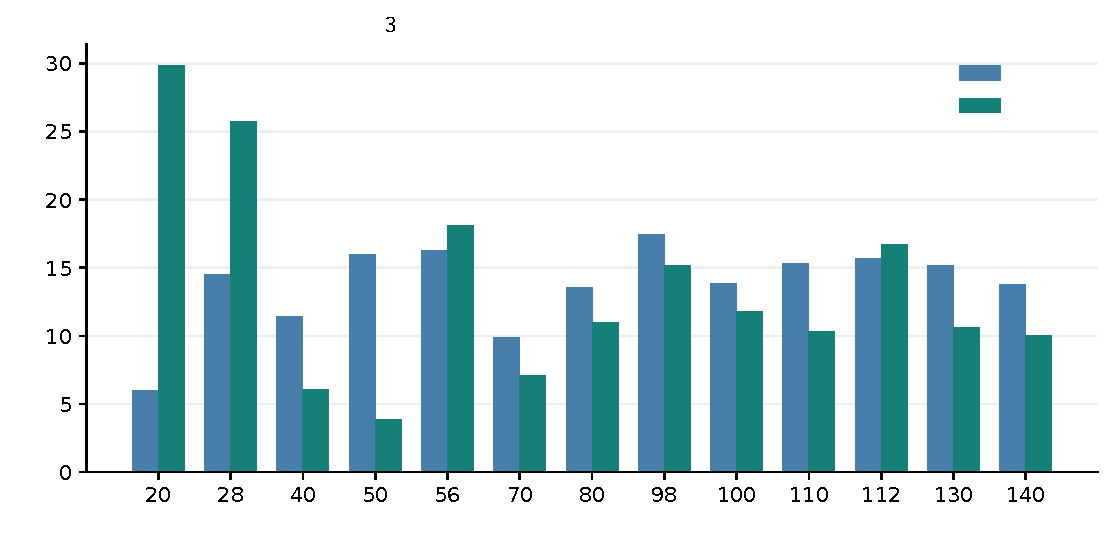
\includegraphics[width=.95\linewidth]{../figures/finite-margins-zh.pdf}\caption{13 个偶数特殊模数的两组非归一化密度分子正性下界。作图数值由精确分数舍入，不是实验数据或优化误差。}\label{zh:margins}\end{figure}
\section{从相位分布到真实时间分布}
上述各构造具有全支撑或正 Haar 成分。紧致相位群上连续向量映射的全支撑均值在其凸包的相对内部：若支撑超平面上的线性泛函在均值处取极值，则连续性和全支撑迫使它处处为常数。对任意正代数数 $\delta$，$\delta c\cdot\alpha\in2\pi\Z$ 当且仅当 $c\cdot\alpha=0$，原因是 $\pi$ 的超越性。由 Kronecker 判据，预设时间网格与连续轨道有相同闭包；非负迭代通过紧致群递归性同样稠密。网格向量的凸包与其闭包有相同相对内部\cite[定理6.3]{rockafellar}，因此存在有限个真实时间及严格正权重。由 Carath\'eodory 定理及字符计数得到定理~\ref{zh:main}的支撑上界。这是存在性结论，不保证实用的最大等待时间。
\section{统一内部裕量与时间噪声}
在完整分类证明的基础上，进一步的移位多项式检验和有限分数比较表明，对每个允许模数可以选取 $\nu\ge h/100$ 的相位概率测度。偶数情形先从每个组 $\nu_b$ 中移除 $ch_b$，$c=1/100$，令 $\rho_b=(\nu_b-ch_b)/(1-c)$。联合分布取 $ch+(1-c)\rho_0\times\rho_1$，组内矩恢复目标，跨组矩保持为零；避免将两个 Haar 比例直接相乘。小模数使用已有相位斜坡构造\cite{kang}或上述 $q=9$ 的混合。全部界的精确检验见 \texttt{verify\_uniform\_floor.py}。

设 $\Omega$ 为不同正 Bohr 频率，目标复矩向量为 $y$（各虚部为零）。对任意 $\sum_\omega|u_\omega|<1/200$，加入 Haar 密度 $2\Rea\sum_\omega u_\omega\bar\chi_\omega$ 即可将复矩移至 $y+u$，同时保持正性和总质量。因此 $y$ 附近有与链长无关的 $\ell^1$ 内部半径 $1/200$。
\begin{corollary}[已知读出时间噪声的补偿，依赖上述分类与裕量]
若独立时间误差 $X$ 分布已知、均值有限、标准差 $\sigma\le1/(25\sqrt N)$，则存在有限计划读出时间分布，使 $\E M(T+X)=J_N/N$。
\end{corollary}
\begin{proof}令 $k_\omega=\E e^{i\omega(X-\E X)}$。由 Taylor 余项 $|k_\omega-1|\le\omega^2\sigma^2/2\le8\sigma^2$，且至多 $N^2/4$ 个目标矩非零、幅度为 $1/N$。因此 $\sum_\omega |y_\omega/k_\omega-y_\omega|\le2N\sigma^2/(1-8\sigma^2)\le2/621<1/200$。再以群平移补偿误差均值，利用凸包内部与时间网格论证，精确实现预补偿矩。独立性保证实际矩恢复为 $y$。\end{proof}
该界使用归一化哈密顿量对应的无量纲时间；对于 $JA$（$\hbar=1$），物理误差标准差需乘以 $|J|$。若要求实际时间非负，误差还需有下界并选足够晚的起始时刻。本推论不是对任意未知噪声的固定协议，也不代表实验验证。
\section{复现与审查状态}
开源资源包保留英文完整详细证明、全部一般矩与误差界程序、有限整数枚举、精确分数及实际运行日志。Python 和 C++ 检查只证明相应有限断言，不能替代一般短关系分类的数学证明。已有 $P_{19}$ Lean 文件仅对应此前的有限整数证书，不覆盖本研究主定理。整个研究采用 AI 辅助推导、代码生成及内部审查，尚未完成独立数学同行评议或 Lean 主定理形式化。本稿不宣称已获正式发表、无误或绝对首创。2026 年 11 月 27 日的定向检索未发现相同完整正向分类，Kang 的强正则图研究\cite{kang2}涉及不同图族。论文详细推导以英文主稿及 DP 为准，中文稿对主要证明链和关键公式进行同步呈现。
\begin{thebibliography}{9}\small
\bibitem{baptista} P. Baptista, G. Coutinho and V. Marques, Unexpected averages of mixing matrices, \emph{Quantum Information Processing} \textbf{23}, 272 (2024). \href{https://doi.org/10.1007/s11128-024-04480-0}{DOI: 10.1007/s11128-024-04480-0}.
\bibitem{kang} M. Kang, Arithmetic of Bohr frequencies governs uniform mixing in randomly timed quantum spin chains, \href{https://arxiv.org/abs/2609.14463}{arXiv:2609.14463v1} (2026), S2--S4.
\bibitem{cj} J. H. Conway and A. J. Jones, Trigonometric diophantine equations (On vanishing sums of roots of unity), \emph{Acta Arithmetica} \textbf{30}, 229--240 (1976). \href{https://doi.org/10.4064/aa-30-3-229-240}{DOI: 10.4064/aa-30-3-229-240}.
\bibitem{lenstra} H. W. Lenstra Jr., Vanishing sums of roots of unity (1979), \href{https://pub.math.leidenuniv.nl/~lenstrahw/PUBLICATIONS/1979d/art.pdf}{原文扫描件}，定理 2.2、2.3、2.6。
\bibitem{rockafellar} R. T. Rockafellar, \emph{Convex Analysis}, Princeton University Press (1970), 定理 6.3、17.1。
\bibitem{godsil} C. Godsil, Average mixing of continuous quantum walks, \emph{J. Combin. Theory Ser. A} \textbf{120}, 1649--1662 (2013). \href{https://doi.org/10.1016/j.jcta.2013.05.006}{DOI: 10.1016/j.jcta.2013.05.006}.
\bibitem{kang2} M. Kang, Moment methods for uniform average mixing on strongly regular graphs, \href{https://arxiv.org/abs/2610.10017}{arXiv:2610.10017} (2026).
\end{thebibliography}
\end{document}
